\documentclass[border=4pt]{standalone}
\usepackage[T1]{fontenc}
\usepackage{mathptmx}
\usepackage{tikz}
\usetikzlibrary{arrows.meta,positioning,fit,backgrounds}
\begin{document}
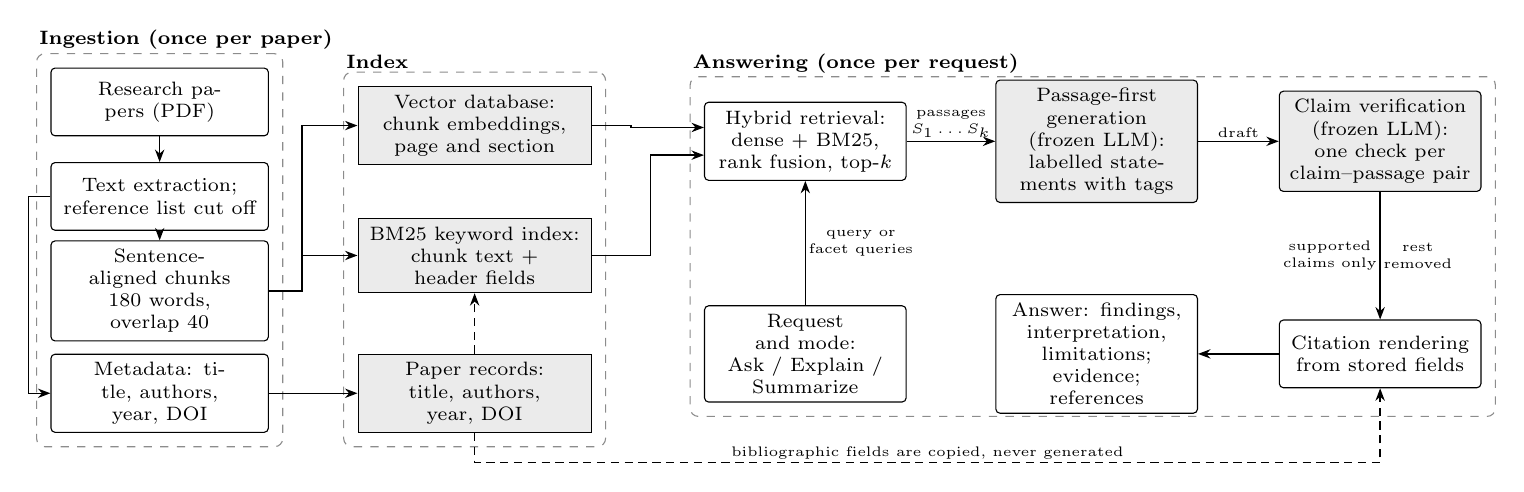
\begin{tikzpicture}[
  font=\scriptsize,
  box/.style={draw, rounded corners=1.5pt, align=center, inner sep=3pt, minimum height=0.86cm, text width=#1},
  box/.default=2.55cm,
  store/.style={draw, align=center, inner sep=3pt, minimum height=0.86cm, text width=2.75cm, fill=black!8},
  llm/.style={box=2.35cm, fill=black!8},
  flow/.style={-{Stealth[length=4.5pt]}, line width=0.5pt},
  note/.style={font=\tiny, align=center, inner sep=1pt},
  lane/.style={draw=black!45, dashed, rounded corners=3pt, inner sep=5pt},
  lanetitle/.style={font=\scriptsize\bfseries, anchor=south west, inner sep=1pt}]
% ---- ingestion
\node[box] (pdf)   at (1.55,4.75) {Research papers (PDF)};
\node[box] (parse) at (1.55,3.55) {Text extraction;\\reference list cut off};
\node[box] (chunk) at (1.55,2.35) {Sentence-aligned chunks\\180 words, overlap 40};
\node[box] (meta)  at (1.55,1.05) {Metadata: title, authors,\\year, DOI};
\draw[flow] (pdf) -- (parse);
\draw[flow] (parse) -- (chunk);
\draw[flow] (parse.west) -- ++(-0.28,0) |- (meta.west);
% ---- index
\node[store] (vec)  at (5.55,4.45) {Vector database:\\chunk embeddings,\\page and section};
\node[store] (bm)   at (5.55,2.80) {BM25 keyword index:\\chunk text + header fields};
\node[store] (rec)  at (5.55,1.05) {Paper records:\\title, authors, year, DOI};
\draw[flow] (chunk.east) -- ++(0.42,0) |- (vec.west);
\draw[flow] (chunk.east) -- ++(0.42,0) |- (bm.west);
\draw[flow] (meta) -- (rec);
\draw[flow, densely dashed] (rec) -- (bm);
% ---- answering
\node[box=2.35cm] (ret)  at (9.75,4.25)  {Hybrid retrieval:\\dense + BM25,\\rank fusion, top-$k$};
\node[llm]        (gen)  at (13.45,4.25) {Passage-first generation\\(frozen LLM): labelled statements with tags};
\node[llm]        (ver)  at (17.05,4.25) {Claim verification\\(frozen LLM): one check per claim--passage pair};
\node[box=2.35cm] (req)  at (9.75,1.55)  {Request and mode:\\Ask / Explain /\\Summarize};
\node[box=2.35cm] (ans)  at (13.45,1.55) {Answer: findings,\\interpretation, limitations;\\evidence; references};
\node[box=2.35cm] (rend) at (17.05,1.55) {Citation rendering\\from stored fields};
\draw[flow] (req) -- node[note, right] {query or\\facet queries} (ret);
\draw[flow] (vec.east) -- ++(0.5,0) |- ([yshift=5pt]ret.west);
\draw[flow] (bm.east) -- ++(0.75,0) |- ([yshift=-5pt]ret.west);
\draw[flow] (ret) -- node[note, above] {passages\\$S_1 \ldots S_k$} (gen);
\draw[flow] (gen) -- node[note, above] {draft} (ver);
\draw[flow] (ver) -- node[note, left] {supported\\claims only} node[note, right] {rest\\removed} (rend);
\draw[flow] (rend) -- (ans);
\draw[flow, densely dashed] (rec.south) -- ++(0,-0.38) -| node[note, pos=0.25, above] {bibliographic fields are copied, never generated} (rend.south);
% ---- lanes
\begin{scope}[on background layer]
\node[lane, fit=(pdf)(meta)(parse)] (l1) {};
\node[lane, fit=(vec)(rec)] (l2) {};
\node[lane, fit=(ret)(ver)(req)(rend)] (l3) {};
\end{scope}
\node[lanetitle] at (l1.north west) {Ingestion (once per paper)};
\node[lanetitle] at (l2.north west) {Index};
\node[lanetitle] at (l3.north west) {Answering (once per request)};
\end{tikzpicture}
\end{document}
